% Reconstruction and unsupervised segmentation results, restyled to match
% architecture_mse.tex and architecture_triplet.tex. Every number is copied
% from Tables 1 and 2 of the paper (arXiv 2303.06367); nothing is re-measured.
% Error bars are +-1 SD: over five seeds for ours, as reported by the cited
% papers for the baselines.
%
%   pdflatex results_segmentation.tex
\documentclass[border=6pt]{standalone}
\usepackage[T1]{fontenc}
\usepackage{helvet}
\renewcommand{\familydefault}{\sfdefault}
\usepackage{amsmath}
\usepackage{pgfplots}
\pgfplotsset{compat=1.18}
\usetikzlibrary{calc}

\definecolor{hcC}{HTML}{6B5B95}     % ours, same hue as the hippocampus in the architecture figures
\definecolor{base}{HTML}{9A968F}    % every baseline; identity carried by marker shape
\definecolor{ink}{HTML}{2B2B2B}
\definecolor{muted}{HTML}{6B6B6B}
\definecolor{grid}{HTML}{E6E4E0}

\pgfplotsset{
  asp/.style={
    width=5.4cm, height=4.6cm, scale only axis=false,
    axis line style={draw=none},
    tick style={draw=none},
    ymajorgrids, xmajorgrids=false, xminorgrids=false, grid style={line width=0.4pt,grid},
    major x grid style={draw=none},
    tick label style={font=\scriptsize,text=muted},
    label style={font=\footnotesize,text=ink},
    title style={font=\footnotesize\bfseries,text=ink,yshift=-2pt},
    every axis plot/.append style={line width=0.8pt},
    error bars/error bar style={line width=0.8pt},
    error bars/error mark options={rotate=90,mark size=2pt,line width=0.8pt},
    clip=false,
  },
  ours/.style={only marks,mark=*,mark size=2.6pt,color=hcC,
               mark options={draw=white,line width=0.6pt,fill=hcC},
               error bars/y dir=both,error bars/y explicit},
  oursopen/.style={only marks,mark=*,mark size=2.6pt,color=hcC,
               mark options={draw=hcC,line width=0.9pt,fill=white},
               error bars/y dir=both,error bars/y explicit},
  basemark/.style={only marks,mark=#1,mark size=3.0pt,color=base,
               mark options={fill=base,draw=white,line width=0.5pt},
               error bars/y dir=both,error bars/y explicit},
}

\begin{document}
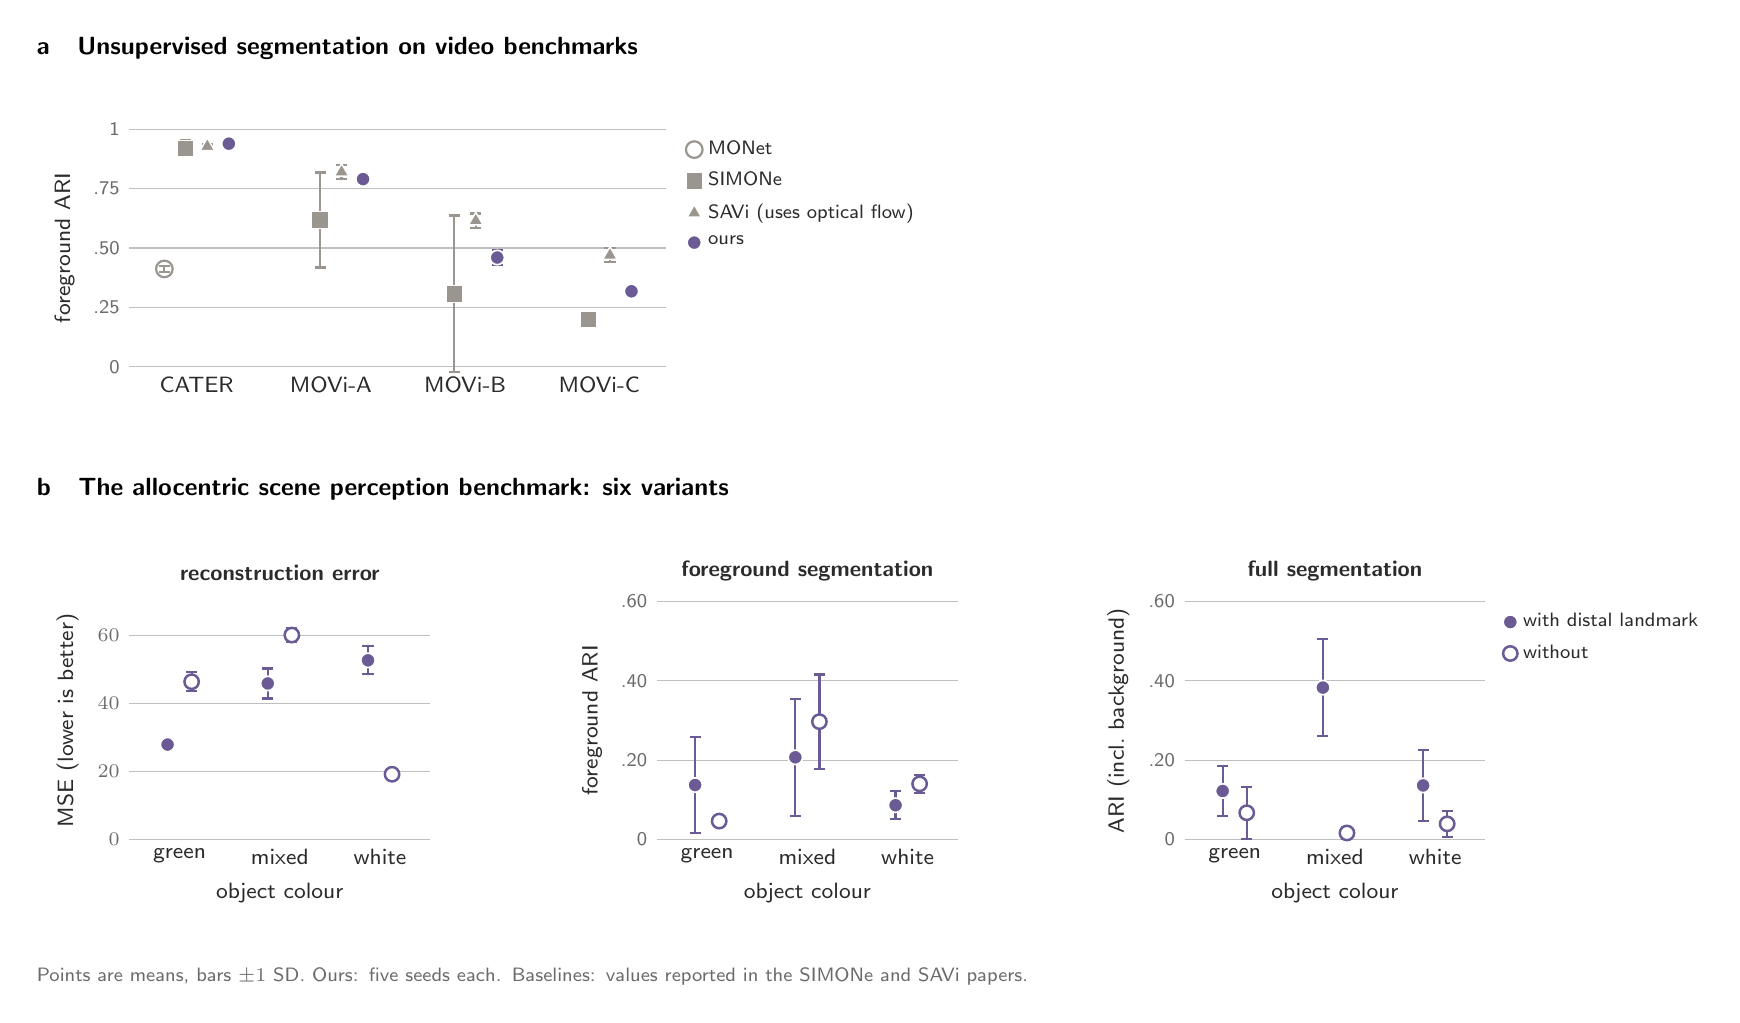
\begin{tikzpicture}[font=\footnotesize]

% ===================================================================== a ===
\node[font=\small\bfseries,anchor=west] at (-1.3,4.05)
  {a\quad Unsupervised segmentation on video benchmarks};
\begin{axis}[asp, width=8.4cm, height=4.6cm,
    at={(0,0)},
    ylabel={foreground ARI}, ymin=0, ymax=1.0, ytick={0,0.25,0.5,0.75,1},
    yticklabels={0,.25,.50,.75,1},
    xmin=0.5, xmax=4.5, xtick={1,2,3,4},
    xticklabels={CATER,MOVi-A,MOVi-B,MOVi-C},
    xticklabel style={font=\footnotesize,text=ink},
    legend style={draw=none,fill=none,font=\scriptsize,text=ink,
                  at={(1.02,1.0)},anchor=north west,row sep=1pt},
    legend cell align=left,
  ]
  % MONet (CATER only)
  \addplot[basemark=o, mark options={fill=white,draw=base,line width=0.8pt}]
    coordinates {(0.76,0.412) +- (0,0.012)};
  % SIMONe
  \addplot[basemark=square*] coordinates {
    (0.92,0.918) +- (0,0.036) (1.92,0.618) +- (0,0.200)
    (2.92,0.307) +- (0,0.330) (3.92,0.198) +- (0,0.005)};
  % SAVi: supervised with optical flow
  \addplot[basemark=triangle*] coordinates {
    (1.08,0.928) +- (0,0.008) (2.08,0.820) +- (0,0.030)
    (3.08,0.615) +- (0,0.030) (4.08,0.470) +- (0,0.030)};
  % ours
  \addplot[ours] coordinates {
    (1.24,0.939) +- (0,0.013) (2.24,0.790) +- (0,0.017)
    (3.24,0.460) +- (0,0.033) (4.24,0.318) +- (0,0.009)};
  \legend{MONet, SIMONe, SAVi (uses optical flow), ours}
\end{axis}

% ===================================================================== b ===
\node[font=\small\bfseries,anchor=west] at (-1.3,-1.55)
  {b\quad The allocentric scene perception benchmark: six variants};

\begin{axis}[asp, at={(0,-6.0cm)}, title={reconstruction error},
    ylabel={MSE (lower is better)}, ymin=0, ymax=70, ytick={0,20,40,60},
    xmin=0.5, xmax=3.5, xtick={1,2,3},
    xticklabels={green,mixed,white}, xticklabel style={font=\footnotesize,text=ink},
    xlabel={object colour},
  ]
  \addplot[ours] coordinates {(0.88,27.912) +- (0,1.289) (1.88,45.908) +- (0,4.405) (2.88,52.713) +- (0,4.119)};
  \addplot[oursopen] coordinates {(1.12,46.411) +- (0,2.777) (2.12,60.159) +- (0,1.923) (3.12,19.167) +- (0,0.575)};
\end{axis}

\begin{axis}[asp, at={(6.7cm,-6.0cm)}, title={foreground segmentation},
    ylabel={foreground ARI}, ymin=0, ymax=0.6, ytick={0,0.2,0.4,0.6},
    yticklabels={0,.20,.40,.60},
    xmin=0.5, xmax=3.5, xtick={1,2,3},
    xticklabels={green,mixed,white}, xticklabel style={font=\footnotesize,text=ink},
    xlabel={object colour},
  ]
  \addplot[ours] coordinates {(0.88,0.137) +- (0,0.122) (1.88,0.207) +- (0,0.148) (2.88,0.086) +- (0,0.035)};
  \addplot[oursopen] coordinates {(1.12,0.046) +- (0,0.010) (2.12,0.297) +- (0,0.119) (3.12,0.140) +- (0,0.023)};
\end{axis}

\begin{axis}[asp, at={(13.4cm,-6.0cm)}, title={full segmentation},
    ylabel={ARI (incl.\ background)}, ymin=0, ymax=0.6, ytick={0,0.2,0.4,0.6},
    yticklabels={0,.20,.40,.60},
    xmin=0.5, xmax=3.5, xtick={1,2,3},
    xticklabels={green,mixed,white}, xticklabel style={font=\footnotesize,text=ink},
    xlabel={object colour},
    legend style={draw=none,fill=none,font=\scriptsize,text=ink,
                  at={(1.03,1.0)},anchor=north west,row sep=1pt},
    legend cell align=left,
  ]
  \addplot[ours] coordinates {(0.88,0.122) +- (0,0.063) (1.88,0.383) +- (0,0.122) (2.88,0.136) +- (0,0.089)};
  \addplot[oursopen] coordinates {(1.12,0.067) +- (0,0.066) (2.12,0.016) +- (0,0.016) (3.12,0.039) +- (0,0.033)};
  \legend{with distal landmark, without}
\end{axis}

\node[font=\scriptsize,text=muted,anchor=west,text width=17cm] at (-1.3,-7.75)
  {Points are means, bars $\pm1$ SD. Ours: five seeds each. Baselines: values reported in the SIMONe and SAVi papers.};
\end{tikzpicture}
\end{document}
